
\documentclass[12pt]{article}
%\setlength{\oddsidemargin}{0in}
%\setlength{\evensidemargin}{0in}
%\setlength{\textwidth}{6.5in}
%\setlength{\parindent}{0in}
%\setlength{\parskip}{\baselineskip}
\thispagestyle{empty}
\usepackage{fullpage}
\usepackage{amsmath,amsthm,amsfonts,empheq}
\usepackage{graphicx, graphics}
\usepackage[usenames,dvipsnames]{color}

\definecolor{darkyellow}{rgb}{.929412,.8314,0}
\definecolor{brightgreen}{rgb}{.439,.824,.0863}

\definecolor{myblue}{rgb}{.8, .8, 1}
\newcommand*\mybluebox[1]{%
\colorbox{myblue}{\hspace{1em}#1\hspace{1em}}}


\newtheorem*{thm}{Theorem}

\begin{document}

%=======================================================
\begin{center}
{\large \bf Comments for Lecture 19}\\
\bf{3.1.2010}
\end{center}



{\bf Notation:} From now on if I write $x\in A$ it means that $x$ is an element of the set $A$.  So for example if I write $x\in \mathbb{R}$ then it means $x$ is a real number.\\

\begin{center}{\LARGE \bf Vector Spaces}.\end{center}

Please review the definition of a vector space (over $\mathbb{R}$) from your notes or the definition given in the book on page 35.  Convince yourself that with our given definitions of vector addition and scalar multiplication in $\mathbb{R}^n$ then  $\mathbb{R}^n$ is a vector space (over $\mathbb{R}$).  This is the vector space we will be focusing on for the time being.  Later in the course we will encounter more general vector spaces but right now you just need to know:

\begin{center} \fbox{$\mathbb{R}^n$ is a vector space (over $\mathbb{R}$) with the vector addition and scalar multiplication we defined.}
\end{center}


\begin{center}{\LARGE \bf Subspaces}.\end{center}

Recall that a subspace is just a vector space that ``lives" in another vector space.

We have also learned a nice shortcut method for determining if something is a subspace of a vector space (see theorem 3.3.2 on p121).

{\bf Example 1:}  The set $W=\{{\bf 0} \}$ (so the set containing only the zero vector ${\bf 0}\in \mathbb{R}^n$) is a subspace of $\mathbb{R}^n$.

{\bf Example 2:}  The set $V=\mathbb{R}^n$ is a subspace of $\mathbb{R}^n$. 

These first two examples of subspaces are not very exiting at all.  We would really like to know if there are any subspaces that are nontrivial (so something other than just the zero vector or all of $\mathbb{R}^n$).

Here is an example of such a subspace:

{\bf Example 3:}  Consider the set $U=\left \{ \left[ \begin{array}{c} x_1  \\ 0  \end{array} \right] \mid x_1 \in \mathbb{R} \right \}$. (Notationally you should read this as ``$U$ is the set of all vectors $\left[ \begin{array}{c} x_1  \\ 0  \end{array} \right]$ such that $x_1$ is some real number.") Here we are thinking of vectors in $\mathbb{R}^2$ as column vectors.  So we want to show that this set $U$ is a subspace of $\mathbb{R}^2$.  Before we knew about theorem 3.3.2 we had to show that $U$ was a subspace by showing it satisfied all ten properties (axioms) of a vector space (p35).  Now we will use our nice shortcut, theorem 3.3.2:

\begin{enumerate}
\item The zero vector ${\bf 0} \in U$ since ${\bf 0} = \left[ \begin{array}{c} 0  \\ 0  \end{array} \right]$ (so here we just made $x_1 = 0$ which is indeed a real number).  Hence ${\bf 0}\in U$.

\item Let ${\bf x}=\left[ \begin{array}{c} x_1  \\ 0  \end{array} \right]$ and let ${\bf y}=\left[ \begin{array}{c} y_1  \\ 0  \end{array} \right]$.  Now notice that

\[ {\bf x} + {\bf y} = \left[ \begin{array}{c} x_1  \\ 0  \end{array} \right] + \left[ \begin{array}{c} y_1  \\ 0  \end{array} \right] = \left[ \begin{array}{c} x_1 + y_1  \\ 0  \end{array} \right] \]

and since $x_1+y_1 \in \mathbb{R}$ then this means ${\bf x} + {\bf y}\in U$.

\item Let ${\bf x}=\left[ \begin{array}{c} x_1  \\ 0  \end{array} \right]$ and let $c\in \mathbb{R}$.  Now notice that 

\[ c{\bf x} = c \left[ \begin{array}{c} x_1  \\ 0  \end{array} \right] = \left[ \begin{array}{c} cx_1  \\ 0  \end{array} \right] \]

and since $cx_1\in \mathbb{R}$ then this means $c{\bf x}\in U$.
\end{enumerate}

So indeed $U$ is a subspace of $\mathbb{R}^2$.


\begin{center}{\LARGE \bf Span}.\end{center}

We say that if $X=\{{\bf v}_1,{\bf v}_2,\ldots,{\bf v}_k \}$ for some collection of vectors where each ${\bf v}_i \in \mathbb{R}^n$ for $1\leq i \leq k$ then:

\begin{empheq}[box=\mybluebox]{align*}
\text{Span}(X)=\{c_1 {\bf v}_1 + c_2 {\bf v}_2 + \ldots + c_k {\bf v}_k \mid c_i \in \mathbb{R}, {\bf v}_i \in X \text{ where } 1\leq i \leq k \}
\end{empheq}

So the $\text{Span}(X)$ is the set of all linear combinations of the vectors from $X$.\\

We have shown that ``the study of spans is the same as the study of subspaces" (this is due to theorems 3.3.1 and 3.3.3).\\

Let's take a look at what we can do with spans.  

{\bf Example 4:}  Let $X = \left\{ \left[ \begin{array}{c} 1  \\ 0  \end{array} \right] \right\}$.  Let's find $\text{Span}(X)$:


\[ \text{Span}(X)= \text{Span} \left( \left \{ \left[ \begin{array}{c} 1  \\ 0  \end{array} \right] \right\} \right) =\left \{c_1 \left[ \begin{array}{c} 1  \\ 0  \end{array} \right] \mid c_1 \in \mathbb{R} \right\} =  \left \{\left[ \begin{array}{c} c_1   \\ 0  \end{array} \right] \mid c_1 \in \mathbb{R} \right\} \]

Remember that the $\text{Span}(X)$ is just a set of vectors.  So for this example we have shown that any vector in $\text{Span}(X)$ has the form $\left[ \begin{array}{c} c_1   \\ 0  \end{array} \right]$ where $c_1$ is any real number.  Do you see that we have encountered this set before?  This set is actually a subspace!  Not only because we have theorem 3.3.1, but take a look at example 3 above.  In example 3 we showed $U=\left \{ \left[ \begin{array}{c} x_1  \\ 0  \end{array} \right] \mid x_1 \in \mathbb{R} \right \}$ is a subspace of $\mathbb{R}^2$, but notice that $\text{Span}(X)=U$.\\

Hopefully this example will help you see the relationship between {\it subspaces} and {\it spans}.  

\begin{center} What can we do with the span? \end{center}

Using theorem 3.3.1 the span gives us a method of constructing subspaces.  We know that $\mathbb{R}^n$ is a vector space.  Now if you are given some collection of vectors in $\mathbb{R}^n$ say $X=\{{\bf v}_1,{\bf v}_2,\ldots,{\bf v}_k \}$ (so you are handed $k$ vectors that live in $\mathbb{R}^n$)  you now have a method for constructing a subspace of $\mathbb{R}^n$ !  Just find $\text{Span}(X)$ and this is a subspace of $\mathbb{R}^n$.  Do you see that constructing a subspace before we introduced the span was not an easy task?  I was only able to ask you if a particular set is a subspace and then you might sigh and go through the tedious details of checking all ten axioms.  Then we learned we only need to check three axioms once we know our collection lives in some vector space.  Now you can not only check if something is a subspace,  you can actually produce subspaces.  The bottom line is that the span is actually not so bad to deal with and it actually is a nice method of producing subspaces.  We will see other methods of creating subspaces as the course continues.\\

Now let's take a closer look at example 4 geometrically:

You start with $\mathbb{R}^2$:

\begin{figure}[h!]
\begin{center} 
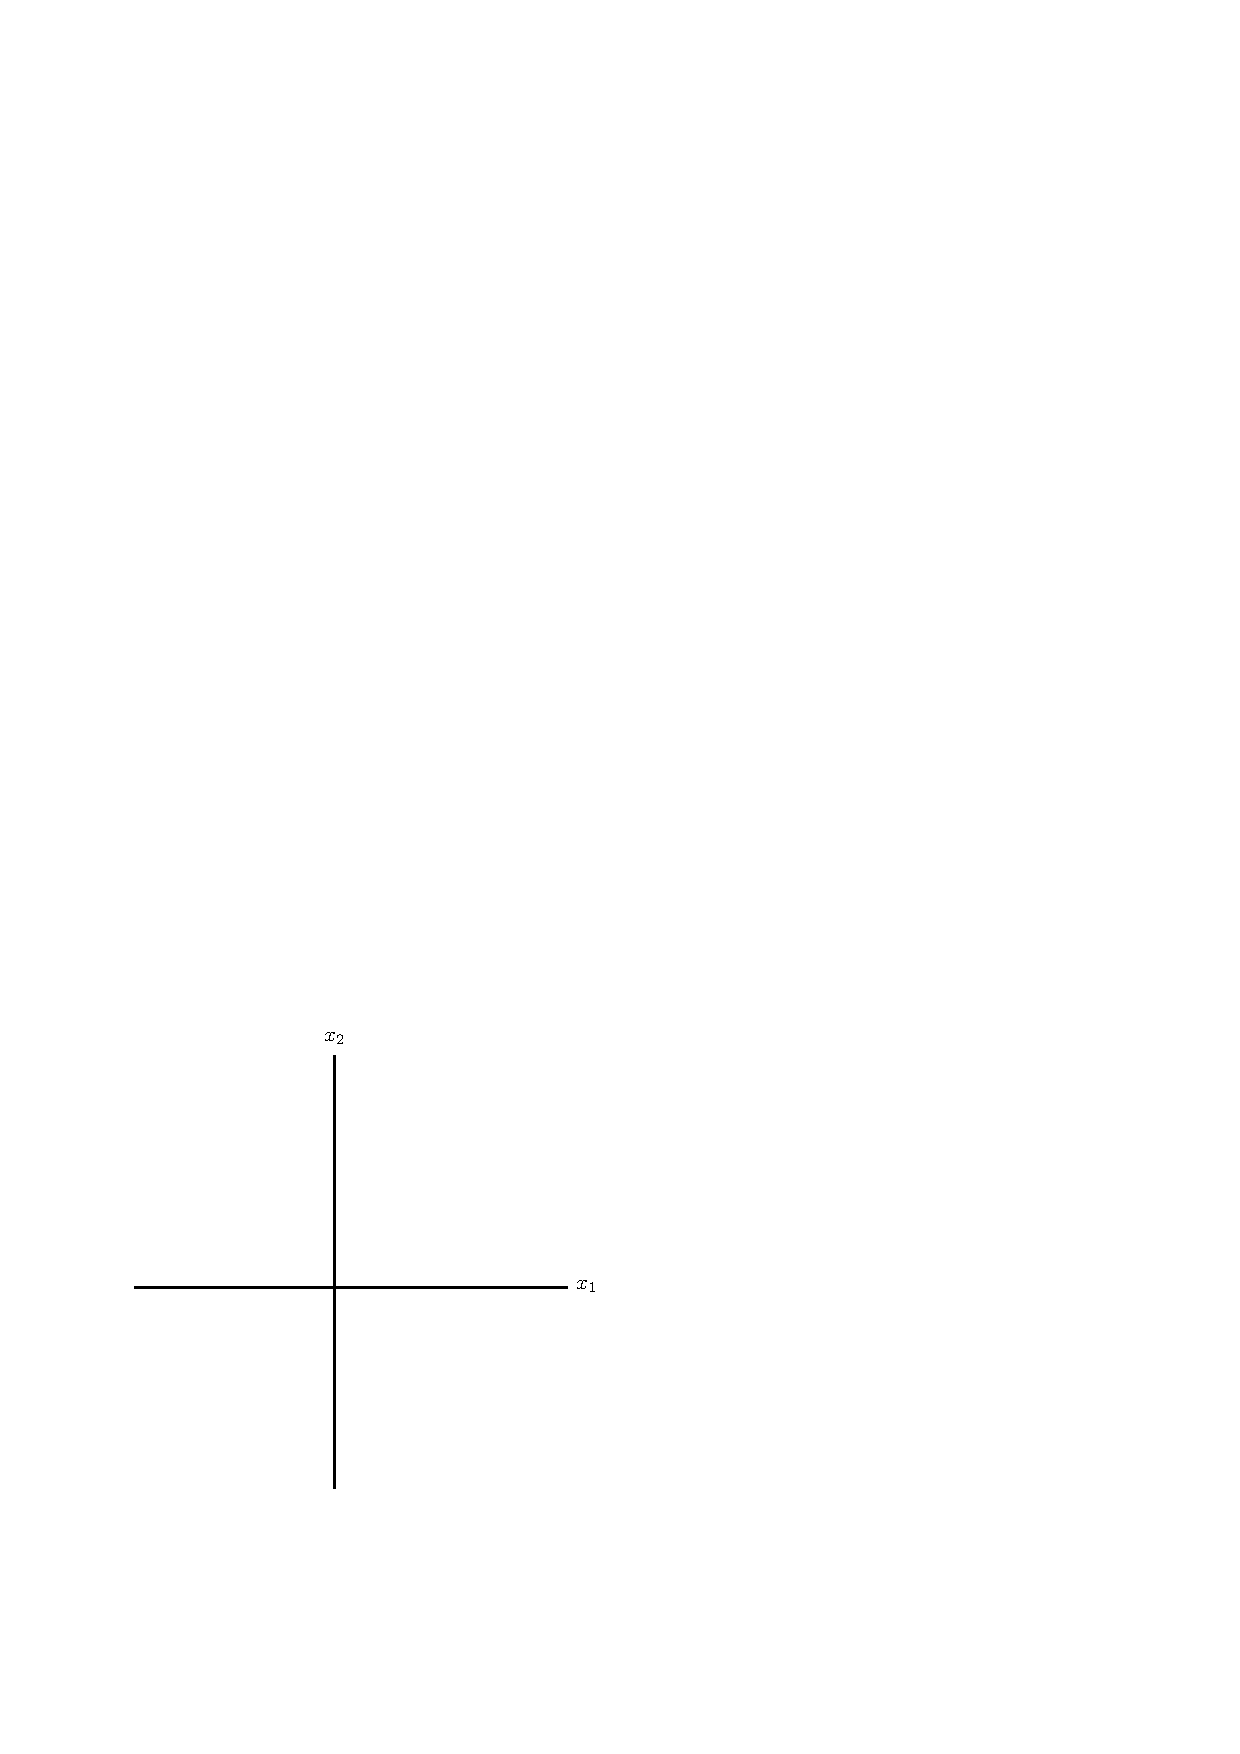
\includegraphics[width=0.25 \textwidth]{l19comim1}
\caption{A lonely and empty Euclidean space $\mathbb{R}^2$.}
\end{center}
\end{figure} 

We have $X= \left\{ \left[ \begin{array}{c} 1  \\ 0  \end{array} \right] \right\}$ (So this is a collection of just one vector in $\mathbb{R}^2$):

\begin{figure}[h!]
\begin{center} 
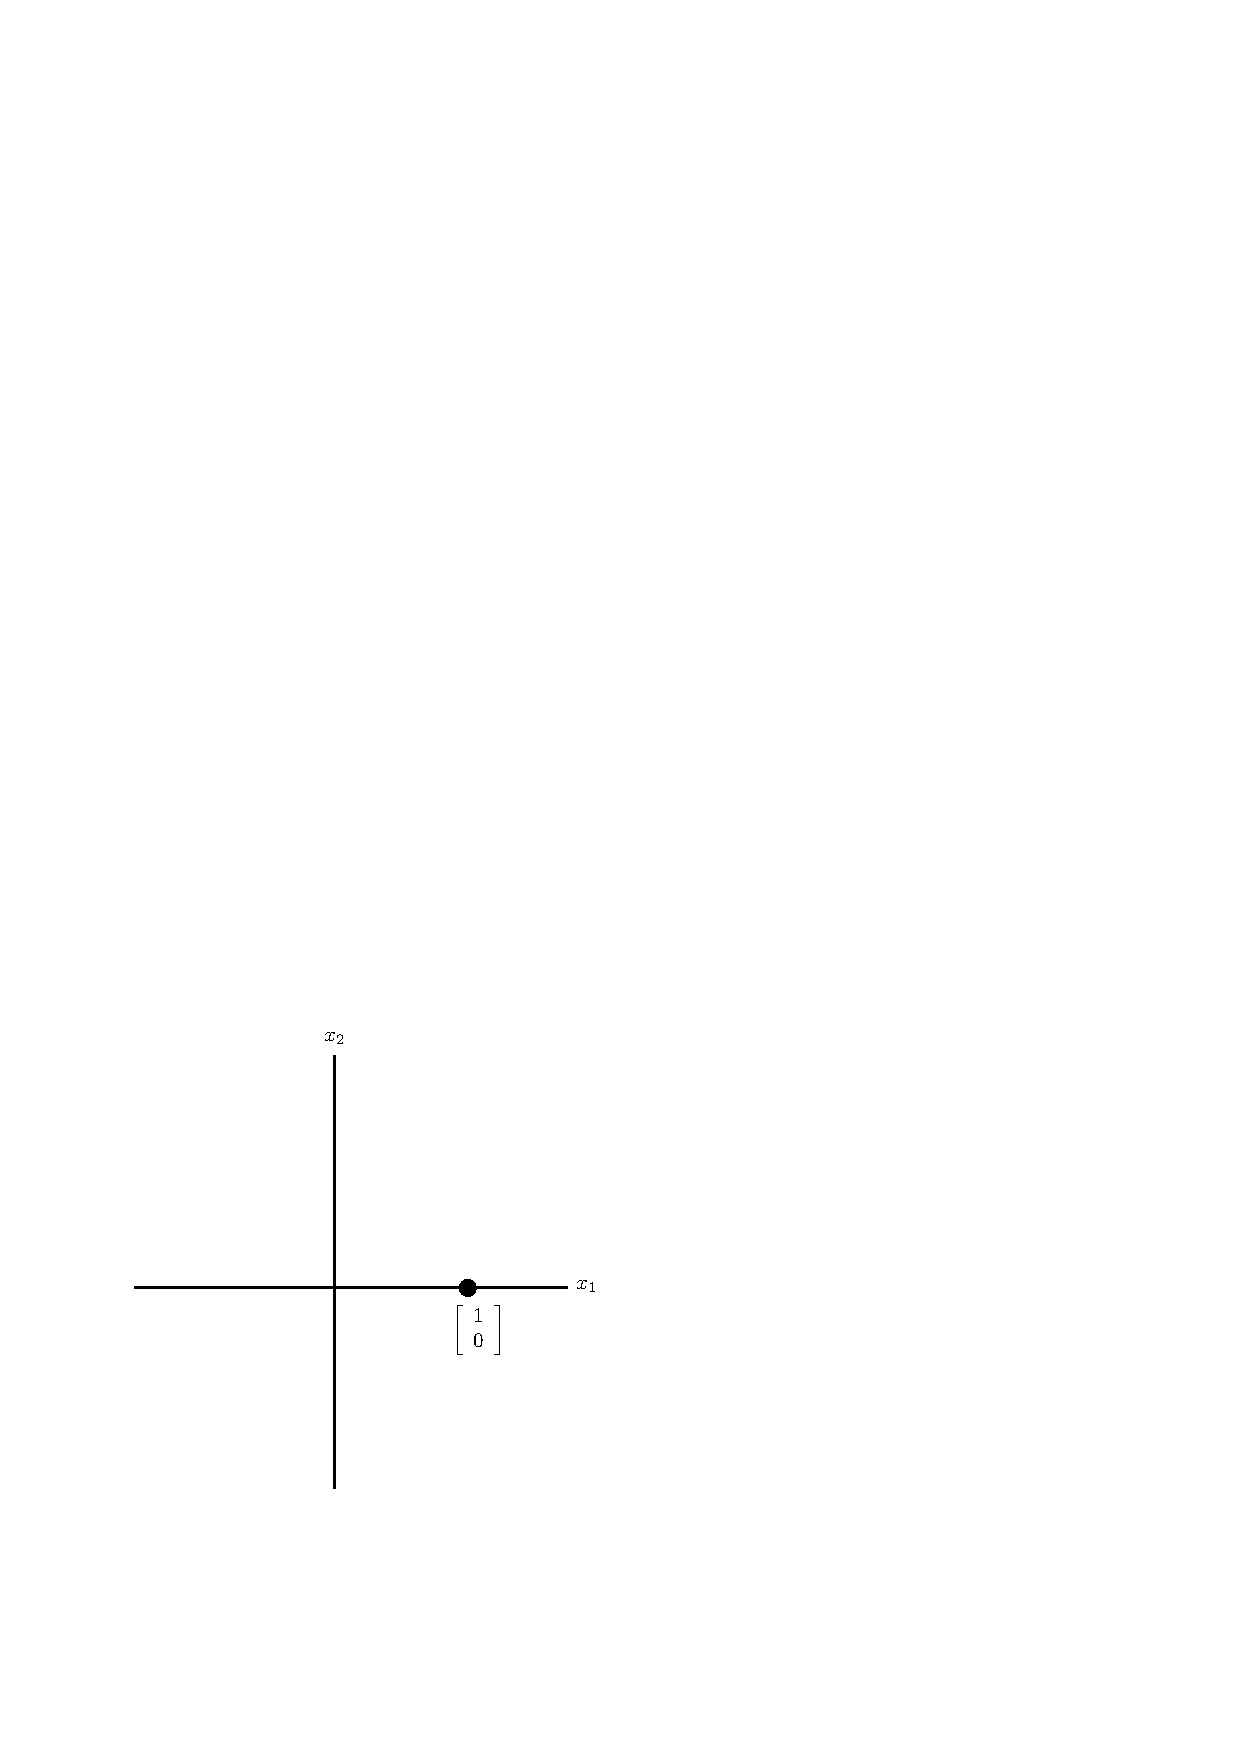
\includegraphics[scale=0.5]{l19comim2}
\caption{The vectors in $X$ join the party.}
\end{center}
\end{figure} 

Now $\text{Span}(X)= \left \{\left[ \begin{array}{c} c_1   \\ 0  \end{array} \right] \mid c_1 \in \mathbb{R} \right\}$ (drawn in red):

\begin{figure}[h!]
\begin{center} 
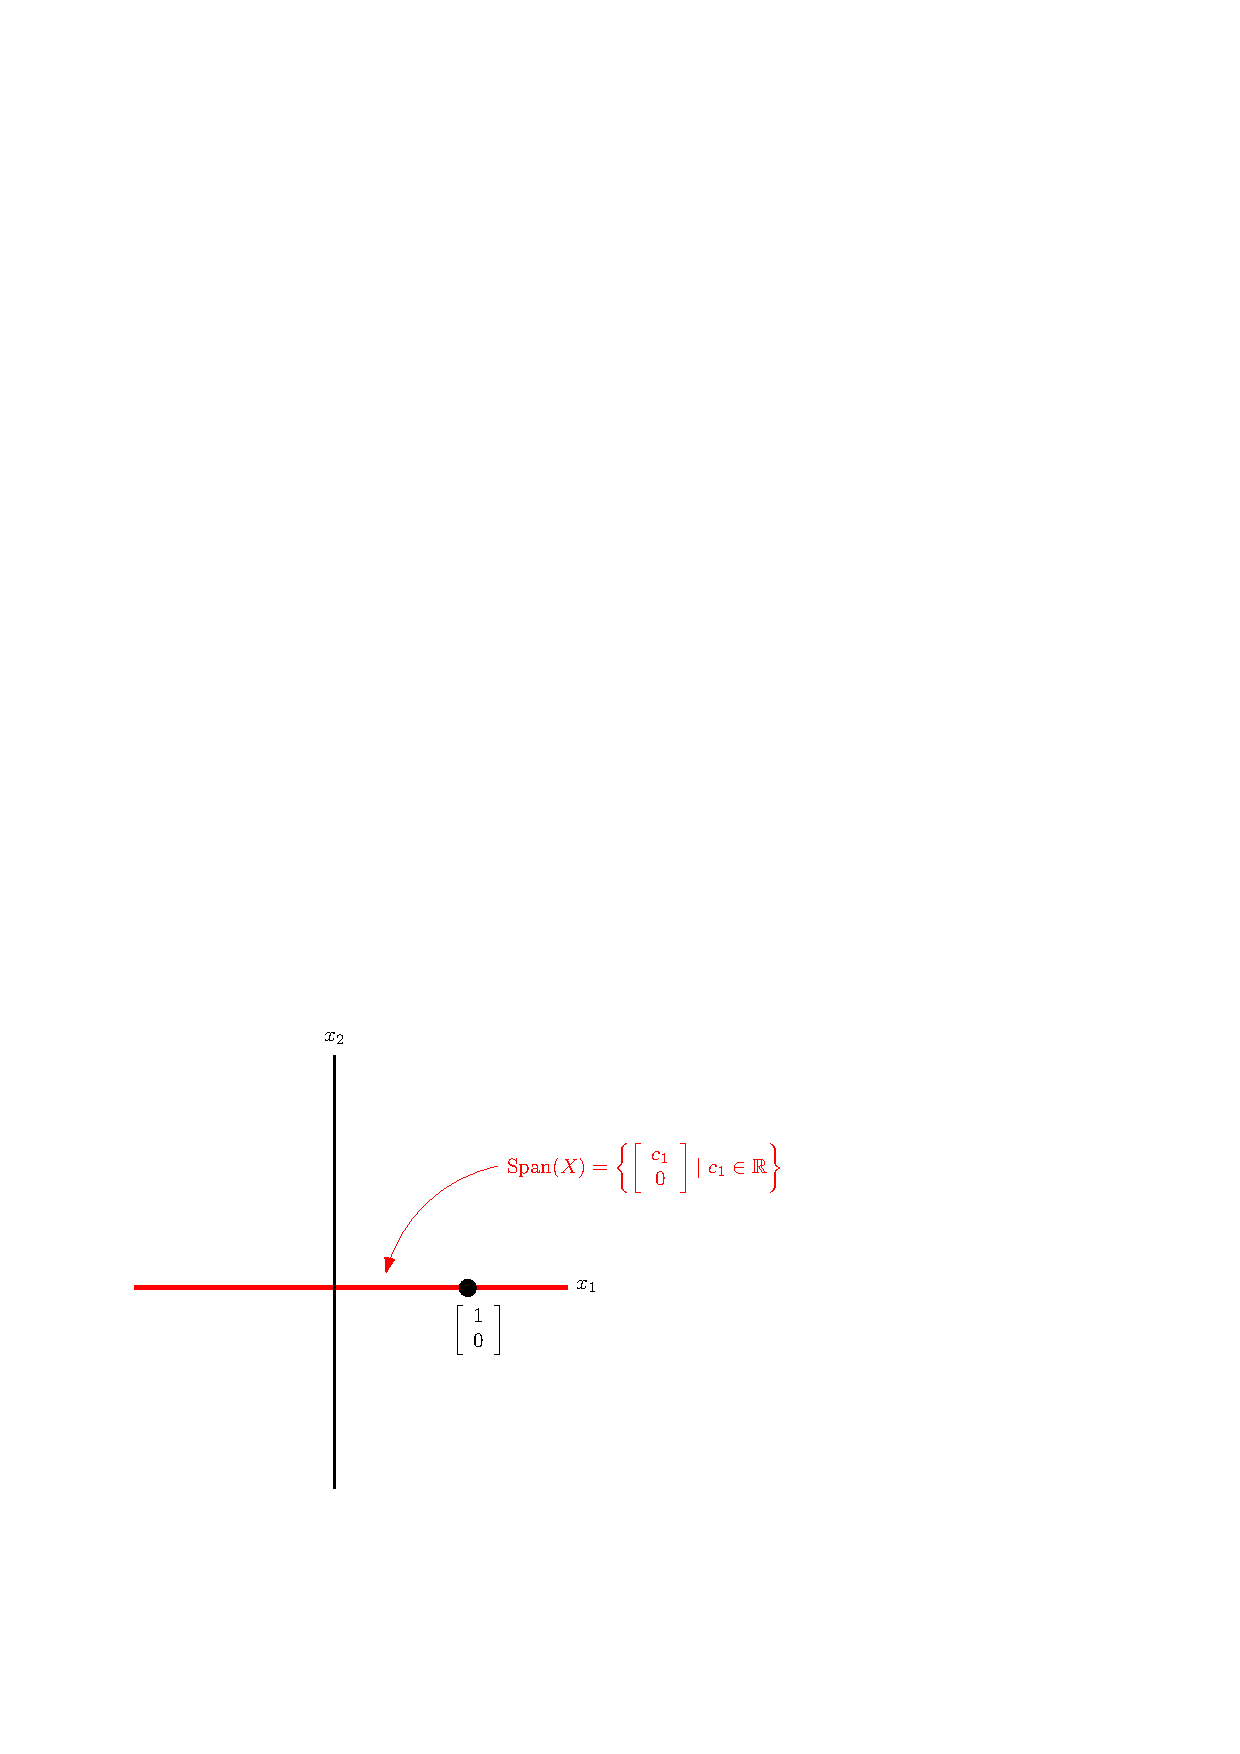
\includegraphics[width=0.6 \textwidth]{l19comim3}
\end{center}
\end{figure} 


Geometrically this is the $x_1$-axis since any point on the $x_1$-axis is of the form $(c_1,0)$ where $c_1\in \mathbb{R}$ so it corresponds to the vector $\left[ \begin{array}{c} c_1  \\ 0  \end{array} \right]$ where  $c_1\in \mathbb{R}$.  Notice of course the vector $\left[ \begin{array}{c} 1  \\ 0  \end{array} \right]$ is in $\text{Span}(X)$ (more generally any vector in $X$ will be in $\text{Span}(X)$ since they are indeed linear combinations of vectors from $X$).

We also know $\text{Span}\left ( \left \{ \left[ \begin{array}{c} 1  \\ 0  \end{array} \right] \right\} \right )$ is a subspace of $\mathbb{R}^2$.  This is our first nontrivial picture of a subspace.  The following problems will help you see the more general picture:

{\bf Problems:}\\
1. In $\mathbb{R}^2$ what would the $\text{Span}(\left \{ \left[ \begin{array}{c} 1  \\ 0  \end{array} \right] , \left[ \begin{array}{c} 0  \\ 1  \end{array} \right]\right\})$ be?  First write this out by definition and think about what the vectors look like both algebraically and geometrically by drawing some pictures (remember things like the parallelogram law). \\

2. In $\mathbb{R}^2$ what would the $\text{Span}\left (\left \{ \left[ \begin{array}{c}  0 \\ 0  \end{array} \right] \right\} \right)$ be? \\

3. In $\mathbb{R}^2$ what would the $\text{Span}\left (\left \{ \left[ \begin{array}{c}  3 \\ 1  \end{array} \right] \right\} \right)$ be? Try to think about this geometrically as well.\\

4. In $\mathbb{R}^2$ what would the $\text{Span}\left (\left \{ \left[ \begin{array}{c}  a \\ b  \end{array} \right] \right\} \right)$ be (where $a$ and $b$ are both in $\mathbb{R}$)?  Try to think about this geometrically as well.\\

5. In $\mathbb{R}^2$ what would the $\text{Span}\left (\left \{ \left[ \begin{array}{c} 1  \\ 1  \end{array} \right] , \left[ \begin{array}{c} 2  \\ 3  \end{array} \right]\right\} \right)$ be?  \\

6. In $\mathbb{R}^2$ what would the $\text{Span}\left (\left \{ \left[ \begin{array}{c} 1  \\ 1  \end{array} \right] , \left[ \begin{array}{c} 2  \\ 2  \end{array} \right]\right\} \right)$ be?  \\

7. In $\mathbb{R}^2$ what would the $\text{Span}\left (\left \{ \left[ \begin{array}{c} 1  \\ 1  \end{array} \right] ,\left[ \begin{array}{c} 0  \\ 1  \end{array} \right] ,\left[ \begin{array}{c} 2  \\ 3  \end{array} \right]\right\} \right)$ be?  \\

8. In $\mathbb{R}^3$ what would the $\text{Span}\left (\left \{ \left[ \begin{array}{c} 1  \\ 0  \\ 0\end{array} \right] , \left[ \begin{array}{c} 0  \\ 1  \\ 0\end{array} \right]\right\} \right)$ be?  First write this out by definition and think about what the vectors look like both algebraically and geometrically by drawing some pictures (remember things like the parallelogram law). \\










%=======================================================


\end{document}
